\section{Preamble}
In this part of this work we define some notations and declare definitions which we will use.
In addition, some former mentioned aspects are being formalized.

Nodes which are contained in a graph are denoted in lower case arabic letters and upper case arabic letters are complete graphs which consist of a set of nodes and a set of edges which connect nodes.
Let $\bigcirc{abc} $ be a circle with $a, b, c $ on its border.
The circle with center $o $ is denoted with $(o) $.
$\triangle{abc} $ is the triangle with corners $a,b $ and $c $.

Furthermore, we assume that there are no four points in any graph which are cocircular since the Delaunay Triangulation is in this case not unique anymore.
This leads to unnecessary case differentiation.

The Unit Disk Graph of a node set $s $ is denoted as $U(s) $.
This graph contains all nodes of node set $s $ and connects two nodes if and only if their distance between each other is at most $1 $.
In addition, we will make use of the so called \emph{Gabriel Graph}, denoted as $GG $. 
It is the graph which contains all nodes of a supergraph $U $ and it contains an edge $uv \in U $ if the Gabriel circle of $uv $ contains no other node.
The Gabriel circle of an edge $uv $ is denoted as $disk(u, v) $.
It is the circle with $u $ and $v $ on its border and with its center on line $uv $. 
In this work $U $ denotes the unit disk graph with unit disk radius $R = 1 $.

Another important graph in order to follow this work is the Partial Delaunay Triangulation (PDT)  \cite{pdt}. It is a planar, t-spanner of the Unit Disk Graph (refer to \ref{PDT}).

The following abbreviations are used throughout this work and introduced here.
\emph{Ready To Send (RTS)} and \emph{Clear To Send (CTS)} describe the process of a node pair to interchange messages while starting the desired topology control, namely PDT and RMYS.

\subsection{Partial Delaunay Triangulation}
\label{PDT}
The Partial Delaunay Triangulation produces a connected, planar, t-spanner of any connected graph in a reactive approach.
No node needs to know its neighborhood.
In this part we will see an example of the reactive construction of $PDT $.
First, we define the Partial Delaunay Triangulation as follows:
\begin{definition}
\label{pdt-def}
An edge $uv \in U $ is in $PDT(U) $ if either 
\begin{enumerate}
\renewcommand{\labelenumi}{(\roman{enumi})}
 \item $uv \in GG $
 \item or $\exists{w} \in U : $ maximizes $\angle{uwv} $, $\bigcirc{uwv}  \backslash \{u, v, w\} = \emptyset $ and $\sin{\angle{uwv}} \geq\frac{|uv|}{R} $, with $R>0 $ being the unit disk radius.
\end{enumerate} 
\end{definition}

The $rPDT $ algorithm taken from chapter 3 of \cite{Xiang-Yang2004} is presented in the following:
\algrenewcommand\algorithmicprocedure{\textbf{}}
\begin{algorithm}\small
\caption{Modified Yao Step}\label{MYS}
\begin{algorithmic}[1]
\Statex \textbf{Input:} any connected graph $G $
\Statex \textbf{Output:} planar, connected graph $G' $

\Statex

\For{each node $p\in G $}
	\State 
\EndFor
\Statex $ G' $ is the subgraph of $G $ consisting of all nodes which are in $G $ and all edges which fulfil that both endpoints of this edge have selected it. 
\end{algorithmic}
\end{algorithm}


For this purpose consider the graph in figure \ref{fig:PDT_1}.


\begin{figure}[h!]
\centering
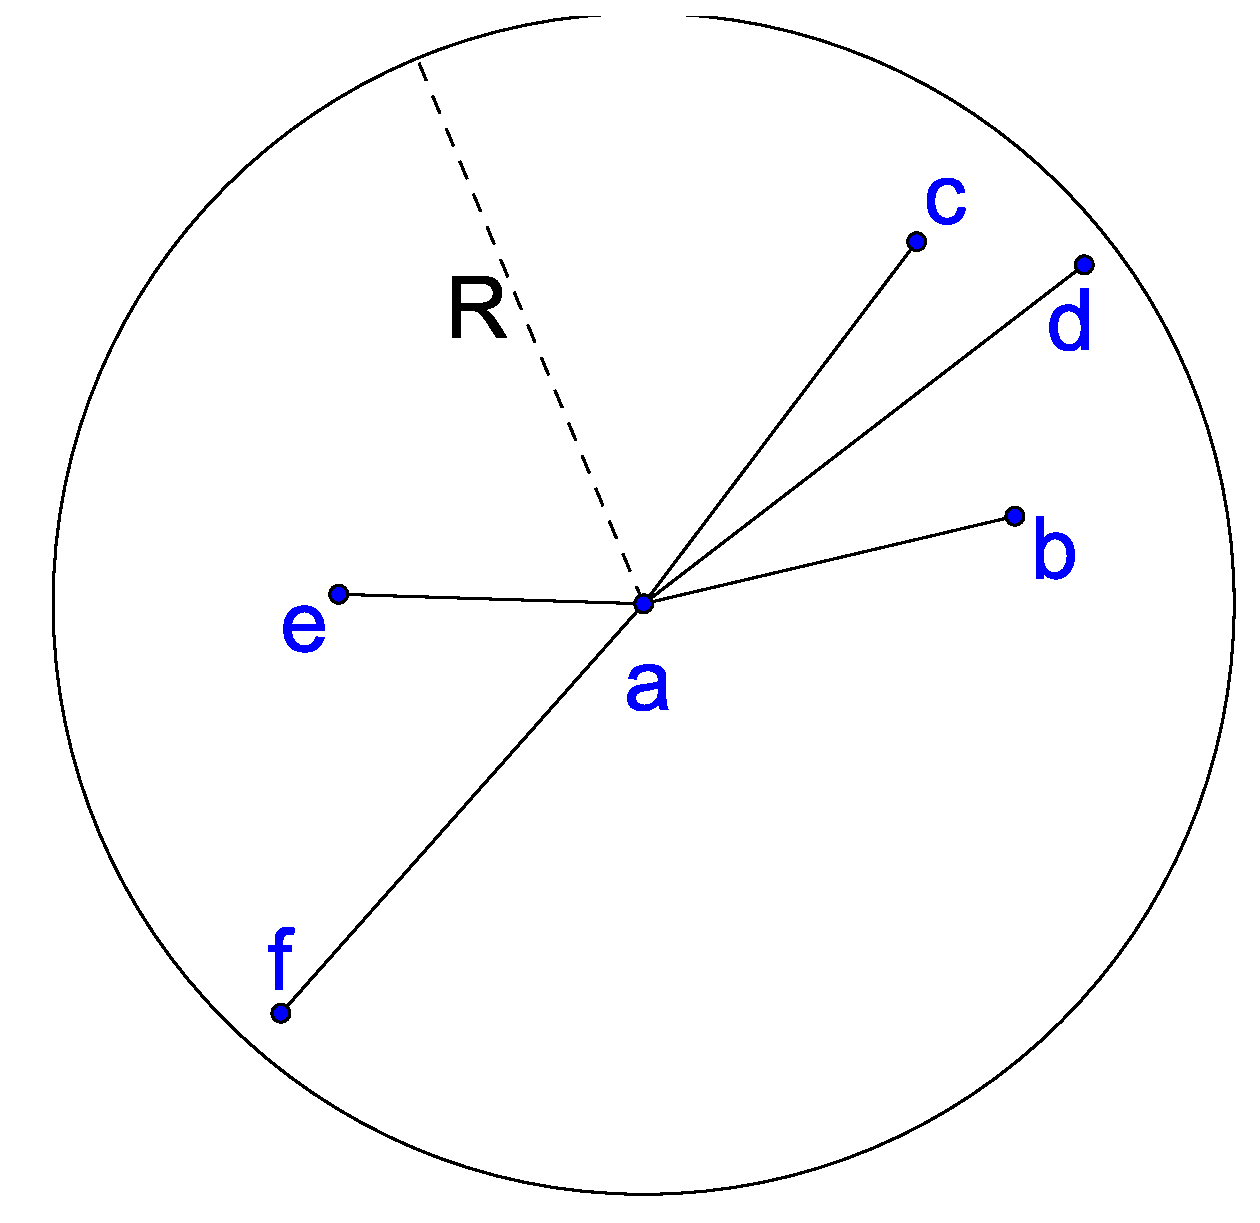
\includegraphics[width=0.5\linewidth]{eps/PDT_1.eps}
\caption{An example graph with unit disk radius $R $ with all edges drawn which are incident on $a $.}
\label{fig:PDT_1}
\end{figure}

